\begin{figure}[htbp]
    \centering
    \begin{subfigure}{0.24\textwidth}
        \centering
        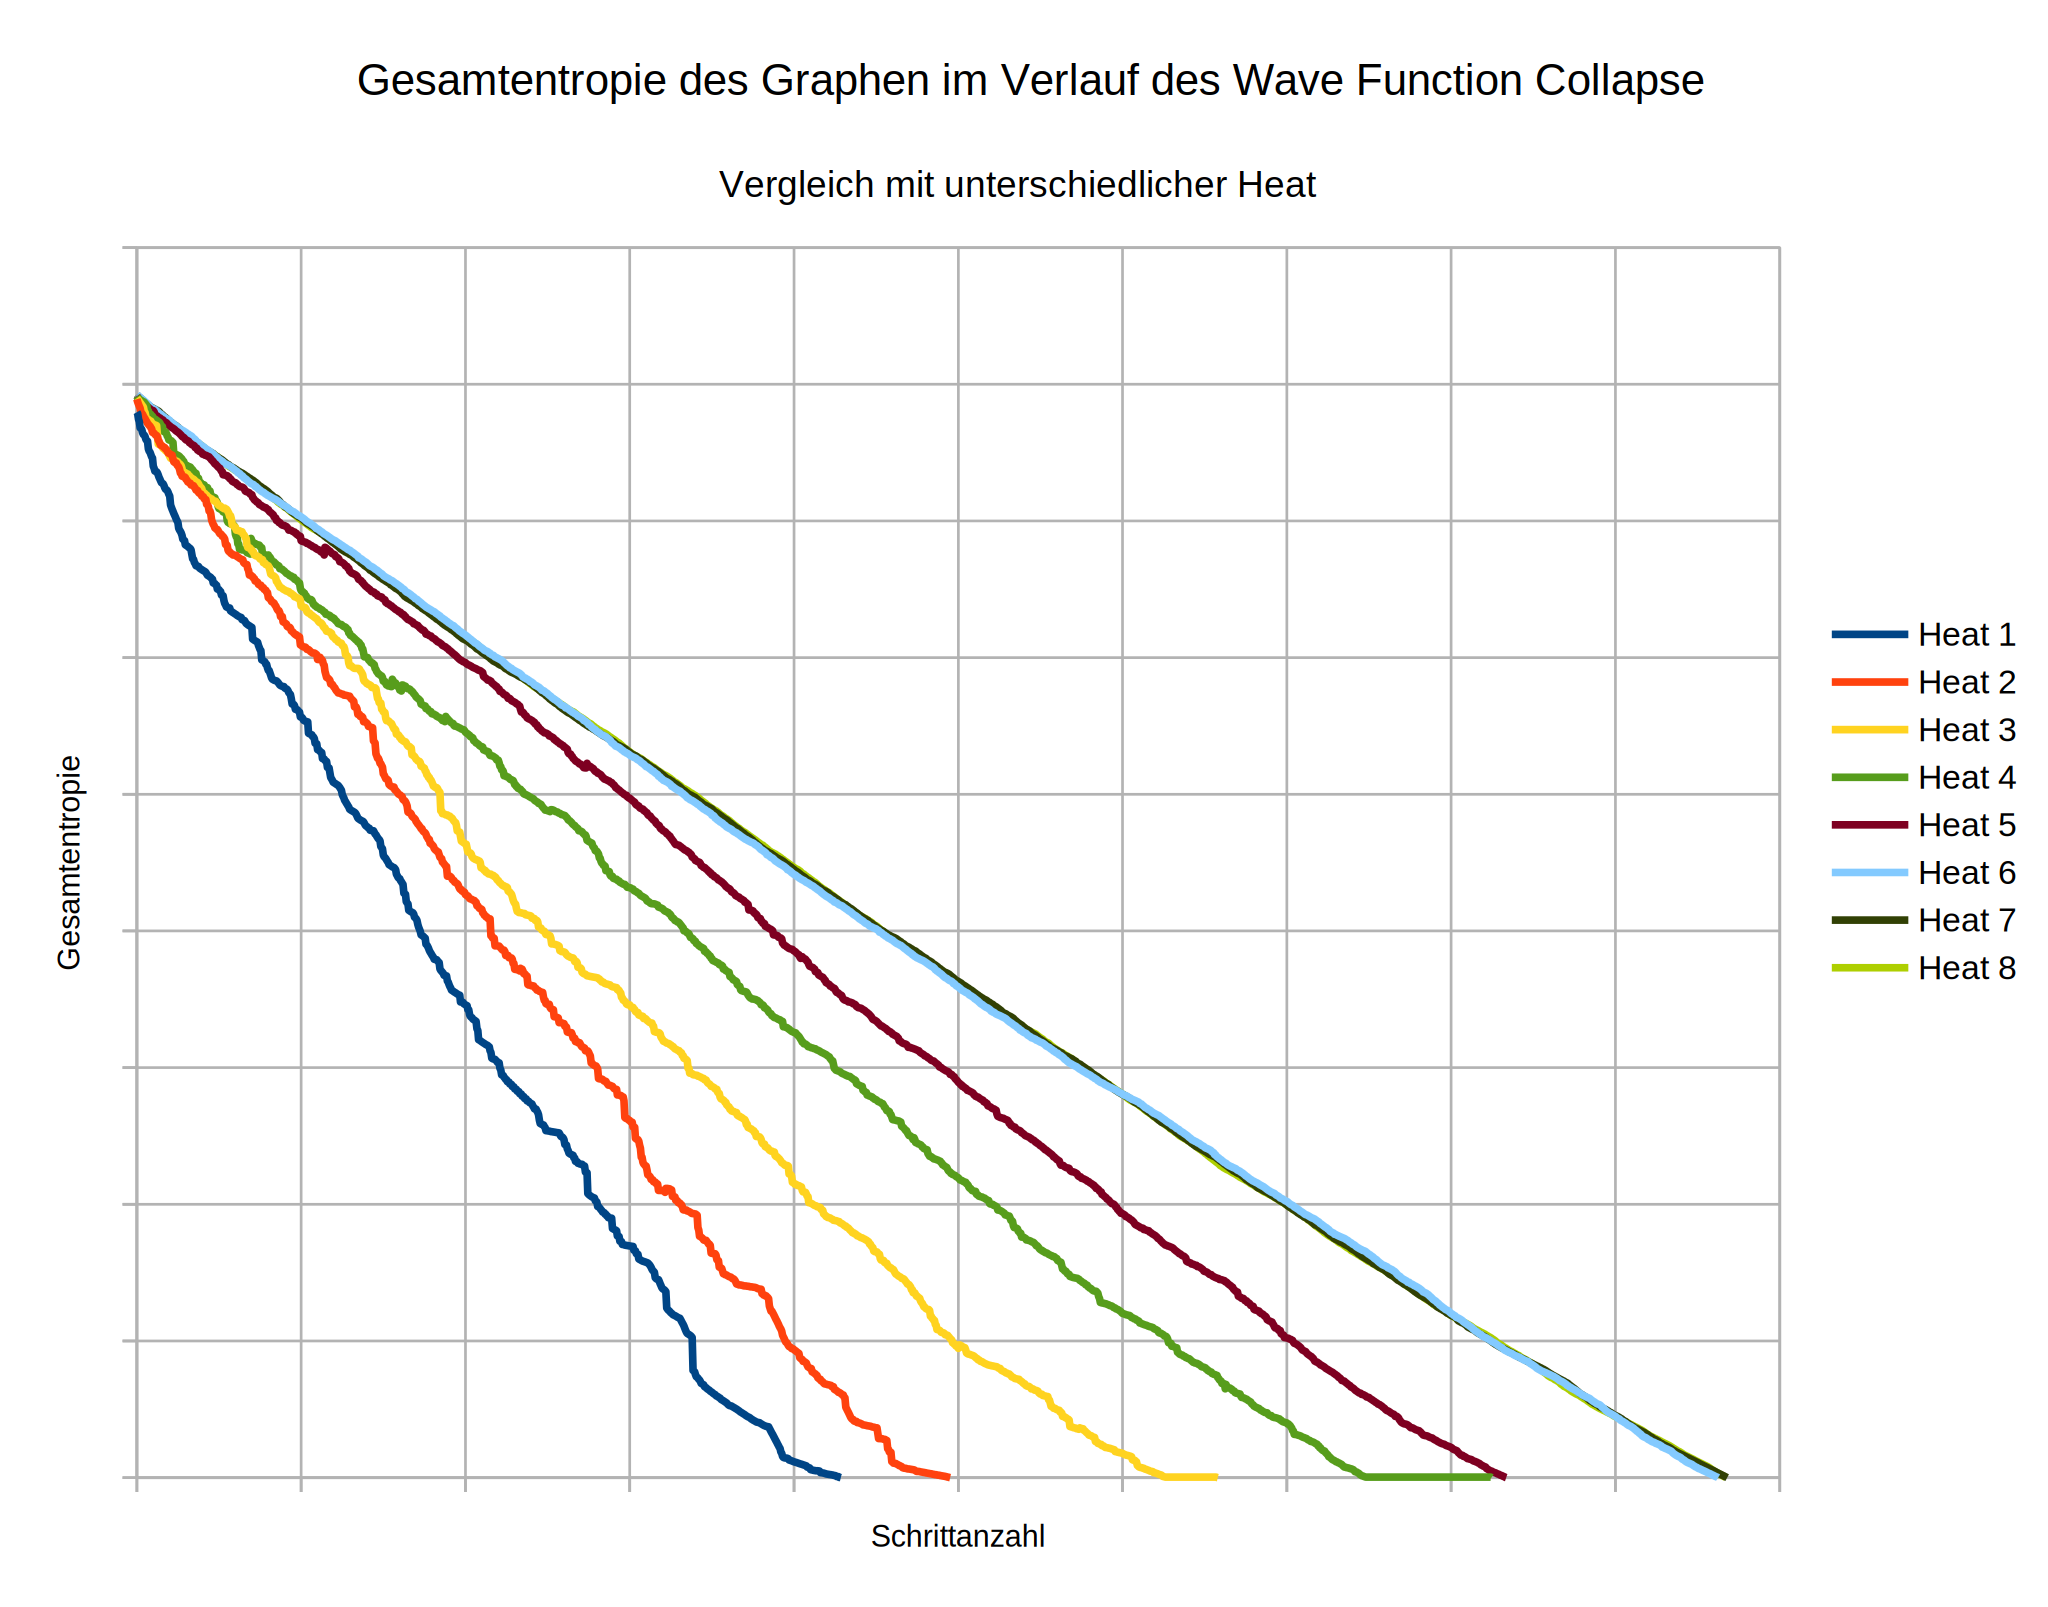
\includegraphics[width=\linewidth]{data/more_heat/1.png}
        \caption{Heat=1}
    \end{subfigure}\hfill
    \begin{subfigure}{0.24\textwidth}
        \centering
        \includegraphics[width=\linewidth]{data/more_heat/2.png}
        \caption{Heat=2}
    \end{subfigure}
    \begin{subfigure}{0.24\textwidth}
        \centering
        \includegraphics[width=\linewidth]{data/more_heat/3.png}
        \caption{Heat=3}
    \end{subfigure}\hfill
    \begin{subfigure}{0.24\textwidth}
        \centering
        \includegraphics[width=\linewidth]{data/more_heat/4.png}
        \caption{Heat=4}
    \end{subfigure}\hfill
        
    \vspace{4mm}
    
    \begin{subfigure}{0.24\textwidth}
        \centering
        \includegraphics[width=\linewidth]{data/more_heat/5.png}
        \caption{Heat=5}
    \end{subfigure}\hfill
    \begin{subfigure}{0.24\textwidth}
        \centering
        \includegraphics[width=\linewidth]{data/more_heat/6.png}
        \caption{Heat=6}
    \end{subfigure}
    \begin{subfigure}{0.24\textwidth}
        \centering
        \includegraphics[width=\linewidth]{data/more_heat/7.png}
        \caption{Heat=7}
    \end{subfigure}\hfill
    \begin{subfigure}{0.24\textwidth}
        \centering
        \includegraphics[width=\linewidth]{data/more_heat/8.png}
        \caption{Heat=8}
    \end{subfigure}\hfill
    
    \caption{
        Beispiele der Generierung bei höherer Heat \at{@incomplete klarmachen, dass es beispielhaft ist und keine Beziehung zwischen den ausgaben außer selbes beispiel und Graph}
    }
    \label{fig:more_heat}
\end{figure}